 %package list
\documentclass{article}
\usepackage[top=3cm, bottom=3cm, outer=3cm, inner=3cm]{geometry}
\usepackage{multicol}
\UseRawInputEncoding
\usepackage{graphicx}
\usepackage{url}
%\usepackage{cite}
\usepackage{hyperref}
\usepackage{array}
%\usepackage{multicol}
\newcolumntype{x}[1]{>{\centering\arraybackslash\hspace{0pt}}p{#1}}
\usepackage{natbib}
\usepackage{pdfpages}
\usepackage{multirow}
\usepackage[normalem]{ulem}
\useunder{\uline}{\ul}{}
\usepackage{svg}
\usepackage{xcolor}
\usepackage{listings}
\lstdefinestyle{ascii-tree}{
    literate={├}{|}1 {─}{--}1 {└}{+}1
  }
\lstset{basicstyle=\ttfamily,
  showstringspaces=false,
  commentstyle=\color{red},
  keywordstyle=\color{blue}
}
%\usepackage{booktabs}
\usepackage{caption}
\usepackage{subcaption}
\usepackage{float}
\usepackage{array}

\newcolumntype{M}[1]{>{\centering\arraybackslash}m{#1}}
\newcolumntype{N}{@{}m{0pt}@{}}

%------------------------------ ÍTEMS --------------------------------

\newcommand{\itemEmail}{hchoquehuancaz@unsa.edu.pe}
\newcommand{\itemStudent}{Hernan Andy Choquehuanca Zapana}
\newcommand{\itemCourse}{Fundamentos de la Programacion II}
\newcommand{\itemCourseCode}{1701213}
\newcommand{\itemSemester}{II}
\newcommand{\itemUniversity}{Universidad Nacional de San Agustin de Arequipa}
\newcommand{\itemFaculty}{Facultad de Ingenieria de Produccion y Servicios}
\newcommand{\itemDepartment}{Departamento Academico de Ingenieria de Sistemas e Informatica}
\newcommand{\itemSchool}{Escuela Profesional de Ingenieria de Sistemas}
\newcommand{\itemAcademic}{2023 - B}
    \newcommand{\itemInput}{Del 10 Enero 2024}
\newcommand{\itemOutput}{Al 15 Enero 2024}
\newcommand{\itemPracticeNumber}{22}
\newcommand{\itemTheme}{Interfaz Gr\'afica de Usuario}

%------------------------------  ------------------------------

\usepackage[english,spanish]{babel}
\usepackage[utf8]{inputenc}
\AtBeginDocument{\selectlanguage{Spanish}}
\renewcommand{\figurename}{Figura}
\renewcommand{\refname}{Referencias}
\renewcommand{\tablename}{Tabla} %esto no funciona cuando se usa babel
\AtBeginDocument{
	\renewcommand\tablename{Tabla}
}

\usepackage{fancyhdr}
\pagestyle{fancy}
\fancyhf{}
\setlength{\headheight}{30pt}
\renewcommand{\headrulewidth}{1pt}
\renewcommand{\footrulewidth}{1pt}
\fancyhead[L]{\raisebox{-0.2\height}{
\includegraphics[width=3cm]{img/logo_episunsa.png}}}
\fancyhead[C]{\fontsize{7}{7}\selectfont	\itemUniversity \\ \itemFaculty \\ \itemDepartment \\ \itemSchool \\ \textbf{\itemCourse}}
\fancyhead[R]{\raisebox{-0.2\height}{
\includegraphics[width=1.2cm]{img/logo_abet}}}
\fancyfoot[L]{Estudiante: Hernan Choquehuanca Zapana}
\fancyfoot[R]{\itemCourse}
\fancyfoot[C]{Página \thepage}

% para el codigo fuente
\usepackage{listings}
\usepackage{color, colortbl}
\definecolor{dkgreen}{rgb}{0,0.6,0}
\definecolor{gray}{rgb}{0.5,0.5,0.5}
\definecolor{mauve}{rgb}{0.58,0,0.82}
\definecolor{codebackground}{rgb}{0.95, 0.95, 0.92}
\definecolor{tablebackground}{rgb}{0.8, 0, 0}

\lstset{frame=tb,
	language=bash,
	aboveskip=3mm,
	belowskip=3mm,
	showstringspaces=false,
	columns=flexible,
	basicstyle={\small\ttfamily},
	numbers=none,
	numberstyle=\tiny\color{gray},
	keywordstyle=\color{blue},
	commentstyle=\color{dkgreen},
	stringstyle=\color{mauve},
	breaklines=true,
	breakatwhitespace=true,
	tabsize=3,
	backgroundcolor= \color{codebackground},
}

%------------------------------ INICIO DEL DOCUMENTO------------------------------

\begin{document}
	
	\vspace*{10px}
	
	\begin{center}	
		\fontsize{17}{17} \textbf{ Informe de Laboratorio \itemPracticeNumber}
	\end{center}
	\centerline{\textbf{\Large Tema: \itemTheme}}
	%\vspace*{0.5cm}	

	\begin{flushright}
		\begin{tabular}{|M{2.5cm}|N|}
			\hline 
			\rowcolor{tablebackground}
			\color{white} \textbf{Nota}  \\
			\hline 
			     \\[30pt]
			\hline 			
		\end{tabular}
	\end{flushright}	

	\begin{table}[H]
		\begin{tabular}{|x{4.7cm}|x{4.8cm}|x{4.8cm}|}
			\hline 
			\rowcolor{tablebackground}
			\color{white} \textbf{Estudiante} & \color{white}\textbf{Escuela}  & \color{white}\textbf{Asignatura}   \\
			\hline 
			{\itemStudent \par \itemEmail} & \itemSchool & {\itemCourse \par Semestre: \itemSemester \par Código: \itemCourseCode}     \\
			\hline 			
		\end{tabular}
	\end{table}		
	
	\begin{table}[H]
		\begin{tabular}{|x{4.7cm}|x{4.8cm}|x{4.8cm}|}
			\hline 
			\rowcolor{tablebackground}
			\color{white}\textbf{Laboratorio} & \color{white}\textbf{Tema}  & \color{white}\textbf{Duración}   \\
			\hline 
			\itemPracticeNumber & \itemTheme & 16 horas   \\
			\hline 
		\end{tabular}
	\end{table}
	
	\begin{table}[H]
		\begin{tabular}{|x{4.7cm}|x{4.8cm}|x{4.8cm}|}
			\hline 
			\rowcolor{tablebackground}
			\color{white}\textbf{Semestre académico} & \color{white}\textbf{Fecha de inicio}  & \color{white}\textbf{Fecha de entrega}   \\
			\hline 
			\itemAcademic & \itemInput &  \itemOutput  \\
			\hline 
		\end{tabular}
	\end{table}


%------------------------------ ACTIVIDADES (TAREA) ------------------------------

	\section{Tarea}
	\begin{itemize}		
        \item Cree una versión del videojuego de estrategia usando componentes básicos GUI: Etiquetas, botones, cuadros de texto, JOptionPane, Color.
        \item Además, utilizar componentes avanzados GUI: Layouts, JPanel, áreas de texto, checkbox, botones de radio y combobox.
        \item Considerar nivel estratégico y táctico.
        \item Considerar hasta las unidades especiales de los reinos.
        \item Hacerlo iterativo.
	\end{itemize}

\newpage

\section{Equipos, materiales y temas utilizados}
	\begin{itemize}
		\item Sistema Operativo Windows 11 Pro 22H2 64 bits.
		\item Visual Studio Code.
		\item Git 2.42.0.
		\item Cuenta en GitHub con el correo institucional.
        \item Editor LaTeX en línea Overleaf.
        \item Herencia.
        \item Polimorfismo.
        \item Miembros de clase.
        \item Clases de Usuario.
        \item Javax.swing.
        \item Java.awt.
        \item Lambda.
        
	\end{itemize}
	
\section{URL de Repositorio Github}
	\begin{itemize}
		\item URL del Repositorio GitHub para clonar o recuperar.
        \item \url{https://github.com/hernanchoquehuanca/fp2-23b.git}
		\item URL para el laboratorio \itemPracticeNumber\ en el Repositorio GitHub.
		\item \url{https://github.com/hernanchoquehuanca/fp2-23b/tree/main/fase03/lab22}
	\end{itemize}

\newpage
 
	\section{Trabajo del Laboratorio \itemPracticeNumber}
        
        
%-----------------------------------------------------------------------------------
%------------------------------------- ACTIVIDADES  --------------------------------
%-----------------------------------------------------------------------------------

% ACTIVIDADESSSS

%\subsection{Actividad 01}

\subsection{Clase VideoJuego.java}
\begin{lstlisting}[language=bash,caption={Commit \href{https://github.com/hernanchoquehuanca/fp2-23b/commit/6cc54a52b073c8adc07ae363b91489277e1490bb}{9575acc}: Concluyendo la clase principal, la cual contiene el main junto con la interfaz gráfica}][H]
 $ git add .
 $ git commit -m "Concluyendo la clase principal en la que se desarrollara el juego"			
 $ git push -u origin main
\end{lstlisting}
\subsubsection{Imports}
\begin{itemize}
    \item \texttt{import java.awt.*;}
    \item \texttt{import java.util.ArrayList;}
    \item \texttt{import javax.swing.*;}
    \item \texttt{import javax.swing.border.EmptyBorder;}
\end{itemize}
\lstinputlisting[language=Java, firstline=1, lastline=5,firstnumber=1,numbers=left]{src/VideoJuego.java}

\subsubsection{Atributos}
\begin{itemize}
    \item \texttt{static boolean turnA = true;}: Para tener un acceso global a ese booleano que sirve como referencia para saber a quien pertenece el turno.
    \item \texttt{public static JButton buttonSel = null;}: Este botón permite tener un guardado del botón presionado, que en nuestro caso sería el soldado seleccionado.
\end{itemize}
\lstinputlisting[language=Java, firstline=7, lastline=9,firstnumber=7,numbers=left]{src/VideoJuego.java}

\subsubsection{Métodos}
\begin{itemize}
    \item \texttt{\textcolor{blue}{main(String[] args)}}: 
    \item Nuestro método principal, en el cual se hace llamado al método startGame() que es quien inicia el juego.
\end{itemize}
\lstinputlisting[language=Java, firstline=10, lastline=12,firstnumber=10,numbers=left]{src/VideoJuego.java}
\newpage 
\begin{itemize}
    \item \texttt{\textcolor{blue}{startGame()}}: 
    \item Este método contiene dentro de sí la ventana inicial, la cual nos da las opciones de Juego 1vs1, Juego personalizado y Salir.
    \item Dentro de este se usa JFrame, JLabel, JButton, JImageIcon y JPanel.
    \item Cada uno de los estos objetos creados cumple para que el diseño de la pagina principal sea la que se muestra a continuación:
\end{itemize}
\begin{figure}[H]
    \centering
    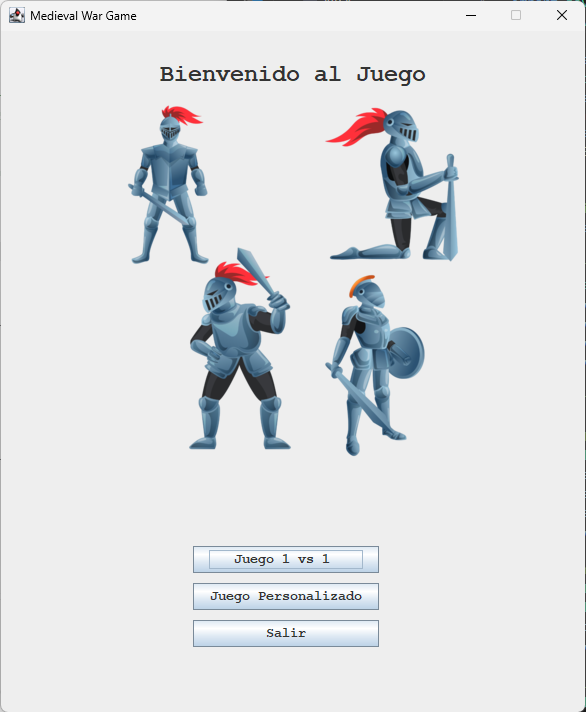
\includegraphics[width=0.71\textwidth,keepaspectratio]{img/vj1.png}
    \caption{}
\end{figure}
\lstinputlisting[language=Java, firstline=15, lastline=76,firstnumber=15,numbers=left]{src/VideoJuego.java}
\begin{itemize}
    \item \texttt{\textcolor{blue}{game1vs1(JFrame w1)}}: 
    \item El método contiene una segunda ventana en la cual se muestra la interfaz del juego de soldados.
    \item Comienza utilizando dispose() para dejar de mostrar la ventana anterior.
    \item Dentro configura la pantalla, agrega los elementos necesarios para el juego y se crean los objetos que permiten la ejecución del juego como: Mapa, Team, Ejercito y Soldado.
    \item Resaltar que se hace uso de funciones lambda, las cuales permiten darle acciones a los botones, además de ayudar al dinamismo del juego.
\end{itemize}
\begin{figure}[H]
    \centering
    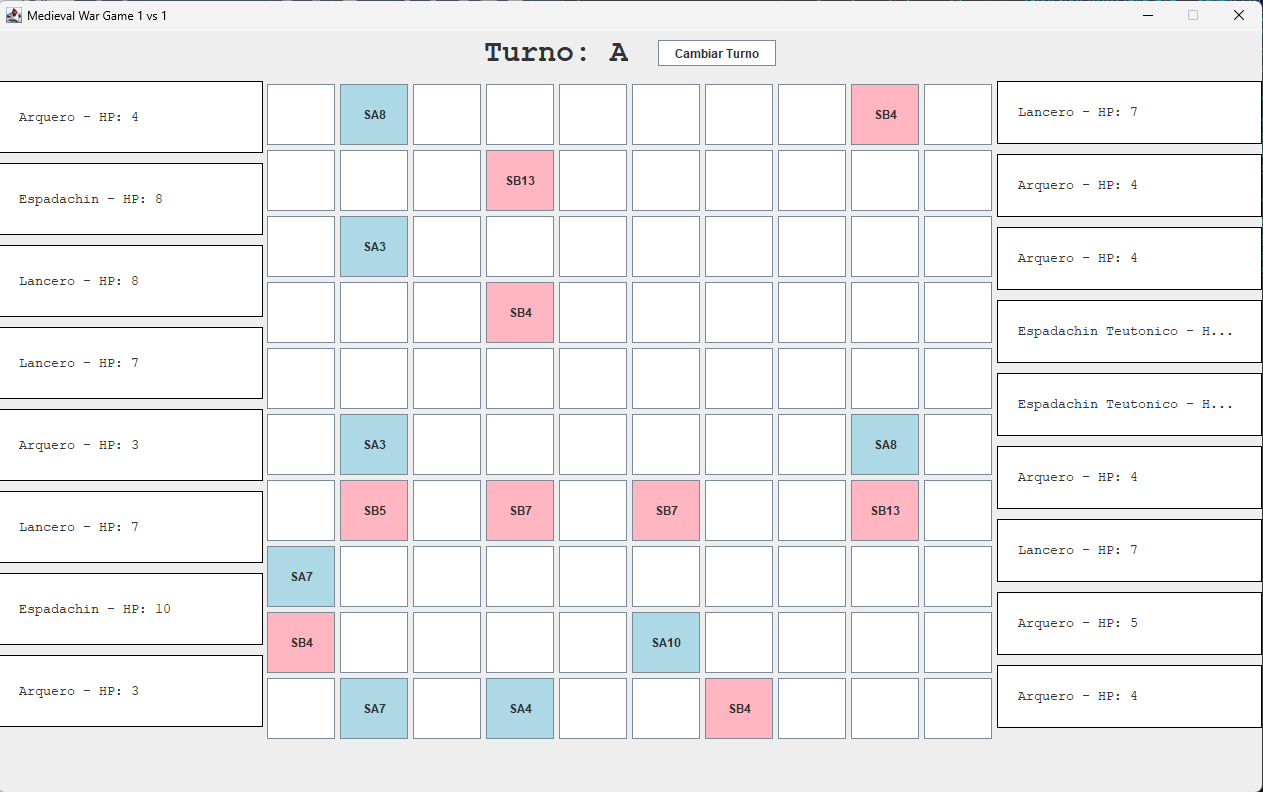
\includegraphics[width=1\textwidth,keepaspectratio]{img/vj2.png}
    \caption{}
\end{figure}
\lstinputlisting[language=Java, firstline=79, lastline=134,firstnumber=79,numbers=left]{src/VideoJuego.java}
\newpage
\begin{itemize}
    \item \texttt{\textcolor{blue}{createJPanelC(Ejercito[][] ejS, Team a, Team b, Mapa map)}}: 
    \item Este método, el cual es usado anteriormente, crea un JPanel el cual va a contener el tablero con los ejércitos ya creados.
    \item Verificando con bucles crea botones según sea el caso, blancos para vacíos, azul para el equipo A y azules para el equipo B.
    \item Haciendo uso de funciones lambda también se le asigna eventos a los botones, estos nos sirven al momento de que el jugador selecciona algún ejército.
\end{itemize}
\lstinputlisting[language=Java, firstline=136, lastline=160,firstnumber=136,numbers=left]{src/VideoJuego.java}
\begin{itemize}
    \item \texttt{\textcolor{blue}{createPanelWE(ArrayList<Ejercito> ej)}}: 
    \item Con este método se crean los paneles del este y oeste del JFrame.
    \item Estos paneles contienen los nombres y el nivel de vida de los ejércitos del team recibido.
    \item De esta manera los jugadores pueden ver con más claridad sus soldados creados.
\end{itemize}
\lstinputlisting[language=Java, firstline=162, lastline=181,firstnumber=162,numbers=left]{src/VideoJuego.java}
\begin{itemize}
    \item \texttt{\textcolor{blue}{armyClick(JButton buttonClicked, JPanel bo, Team a, Team b, Mapa map)}}: 
    \item Este método tiene la finalidad de realizar el combate entre los ejércitos seleccionados.
    \item Se usa un botón atacante y uno atacado, luego con el método fight() se decide el ganador.
\end{itemize}
\lstinputlisting[language=Java, firstline=183, lastline=193,firstnumber=183,numbers=left]{src/VideoJuego.java}
\begin{itemize}
    \item \texttt{\textcolor{blue}{changeTurn(boolean turnA)}}: 
    \item Al ser llamado su función es retornar el booleano opuesto al ya obtenido, para de esta manera tener controlado los turnos de jugadores.
\end{itemize}
\begin{figure}[H]
    \centering
    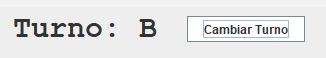
\includegraphics[width=0.3\textwidth,keepaspectratio]{img/vj3.png}
    \caption{}
\end{figure}
\lstinputlisting[language=Java, firstline=195, lastline=197,firstnumber=195,numbers=left]{src/VideoJuego.java}
\begin{itemize}
    \item \texttt{\textcolor{blue}{fight(JPanel game, JButton attacker, JButton attacked, Team a, Team b, Mapa m)}}: 
    \item Haciendo uso del nivel de la suma de vida de los ejércitos de la pelea, se usan probabilidades para determinar el ganador y perdedor.
    \item el perdedor es borrado del tablero, mientras que el ganador en caso se pueda, va a la posición del derrotado o se queda en la misma si fue el atacado.
\end{itemize}
\lstinputlisting[language=Java, firstline=199, lastline=244,firstnumber=199,numbers=left]{src/VideoJuego.java}
\newpage
\begin{itemize}
    \item \texttt{\textcolor{blue}{endWar(Soldado[][] bo)}}: 
    \item Su única función es verificar que alguno de los dos equipos se quede sin ejércitos, en caso pase devuelve true.
\end{itemize}
\lstinputlisting[language=Java, firstline=250, lastline=262,firstnumber=250,numbers=left]{src/VideoJuego.java}
\begin{itemize}
    \item \texttt{\textcolor{blue}{showWinner(Soldado[][] bo)}}: 
    \item El método tiene la misma lógica del anterior, pero en este caso muestra en pantalla al team ganador y finaliza el programa.
\end{itemize}
\lstinputlisting[language=Java, firstline=264, lastline=279,firstnumber=264,numbers=left]{src/VideoJuego.java}
\begin{figure}[H]
    \centering
    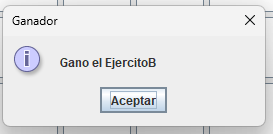
\includegraphics[width=0.3\textwidth,keepaspectratio]{img/vj5.png}
    \caption{}
\end{figure}

%%%%
\newpage

\subsection{Clase Team.java}
\begin{lstlisting}[language=bash,caption={Commit \href{https://github.com/hernanchoquehuanca/fp2-23b/commit/b88b62a5f399f7d5f245434c901abf128f9c0705}{b88b62a}: Agregando la clase Team
}][H]
 $ git add .
 $ git commit -m "Agregada la clase Team, objeto que contendra a los ejercitos"			
 $ git push -u origin main
\end{lstlisting}
\subsubsection{Imports}
\begin{itemize}
    \item \texttt{import java.util.ArrayList;}: 
\end{itemize}
\lstinputlisting[language=Java, firstline=1, lastline=1,firstnumber=1,numbers=left]{src/Team.java}

\subsubsection{Atributos}
\begin{itemize}
    \item \texttt{ArrayList<Ejercito> teams}: Contiene a los ejércitos de un equipo.
    \item \texttt{int numArmy}: Contiene el número de Ejércitos que hay en el equipo.
\end{itemize}
\lstinputlisting[language=Java, firstline=4, lastline=5,firstnumber=4,numbers=left]{src/Team.java}

\subsubsection{Métodos}
\begin{itemize}
    \item \texttt{\textcolor{blue}{Team (Mapa map, char name)}}: 
    \item En el constructor se crean los Ejércitos del equipo, además que se van almacenando en el atributo tipo ArrayList de Ejercito.
\end{itemize}
\lstinputlisting[language=Java, firstline=7, lastline=15,firstnumber=7,numbers=left]{src/Team.java}
\begin{itemize}
    \item \texttt{\textcolor{blue}{getTeams()}}: 
    \item Además del método para obtener el ArrayList de Ejercito.
\end{itemize}
\lstinputlisting[language=Java, firstline=17, lastline=19,firstnumber=17,numbers=left]{src/Team.java}
\newpage
\begin{itemize}
    \item \texttt{\textcolor{blue}{createArmy (Mapa map, char n)}}: 
    \item Sirve para crear a los elementos Ejercito del equipo, genera sus posiciones en el mapa y va seteando algunos atributos de los ejércitos.
\end{itemize}
\lstinputlisting[language=Java, firstline=21, lastline=35,firstnumber=21,numbers=left]{src/Team.java}

%%%%
\newpage
\subsection{Clase Mapa.java}
\begin{lstlisting}[language=bash,caption={Commit \href{https://github.com/hernanchoquehuanca/fp2-23b/commit/1a0586ff7f8bb3b99f7e0c7a74e9bb209487b2c5}{379f06f}: Terminada la clase mapa
}][H]
 $ git add .
 $ git commit -m "Terminada la clase mapa"			
 $ git push -u origin main
\end{lstlisting}
\subsubsection{Imports}
\begin{itemize}
    \item \texttt{import java.util.Arrays;}: 
    \item \texttt{import java.util.List;}: 
\end{itemize}
\lstinputlisting[language=Java, firstline=1, lastline=2,firstnumber=1,numbers=left]{src/Mapa.java}

\subsubsection{Atributos}
\begin{itemize}
    \item \texttt{static Mapa instanciaSingleton}: Crea el mapa de juego haciendo uso de Singleton.
    \item \texttt{String[] typesTerritory}: Contiene todos los posibles territorios que se pueden tener.
    \item \texttt{String territory}: Contiene el tipo de territorio del mapa actual.
    \item \texttt{Ejercito[][] board}: Contiene el tablero de soldados de ambos ejércitos.
\end{itemize}
\lstinputlisting[language=Java, firstline=4, lastline=7,firstnumber=4,numbers=left]{src/Mapa.java}

\subsubsection{Métodos}
\begin{itemize}
    \item \texttt{\textcolor{blue}{getInstance()}}: 
    \item Usamos Singleton para no crear nuevos mapas y asi usar la misma instancia cuando se quiera jugar de nuevo.
\end{itemize}
\lstinputlisting[language=Java, firstline=9, lastline=15,firstnumber=9,numbers=left]{src/Mapa.java}
\begin{itemize}
    \item \texttt{\textcolor{blue}{Getters y Setters}}: 
    \item Además del método para generar un territorio random.
\end{itemize}
\lstinputlisting[language=Java, firstline=17, lastline=40,firstnumber=9,numbers=left]{src/Mapa.java}
\begin{itemize}
    \item \texttt{\textcolor{blue}{addArmy(Soldado s, int r, int c)}}: 
    \item Sirve para agregar Ejercitos al tablero del mapa.
\end{itemize}
\lstinputlisting[language=Java, firstline=42, lastline=44,firstnumber=42,numbers=left]{src/Mapa.java}
\begin{itemize}
    \item \texttt{\textcolor{blue}{checkArmy(int r, int c)}}: 
    \item Verifica si existe o no un Ejercito en la posición recibida.
\end{itemize}
\lstinputlisting[language=Java, firstline=46, lastline=48,firstnumber=46,numbers=left]{src/Mapa.java}
\begin{itemize}
    \item \texttt{\textcolor{blue}{editDeleteBoard(int r, int c)}}: 
    \item Elimina Ejercitos del tablero, útil para los enfrentamientos donde los Ejercito perdedores se eliminan.
\end{itemize}
\lstinputlisting[language=Java, firstline=50, lastline=52,firstnumber=50,numbers=left]{src/Mapa.java}

%%%%

\subsection{Clase Ejercito.java}
\begin{lstlisting}[language=bash,caption={Commit \href{https://github.com/hernanchoquehuanca/fp2-23b/commit/94bd50accf6a9c7aaf3aebd286fbfba93da2e5d8}{94bd50a}: Redefiniendo la clase Ejercito, adaptando y reorganizando su contenido}][H]
 $ git add .
 $ git commit -m "Redefiniendo la clase Ejercito, adaptando y reorganizando su contenido"			
 $ git push -u origin main
\end{lstlisting}
\subsubsection{Imports}
\begin{itemize}
    \item \texttt{import java.util.ArrayList;}
\end{itemize}
\lstinputlisting[language=Java, firstline=1, lastline=1,firstnumber=1,numbers=left]{src/Ejercito.java}

\subsubsection{Atributos}
\begin{itemize}
    \item \texttt{String kingdom}: Contiene el tipo de reino que le tocó al ejército.
    \item \texttt{char name}: Contiene el char identificador ('A' o 'B').
    \item \texttt{ArrayList<Soldado> army}: Guarda a los soldados creados.
\end{itemize}
\lstinputlisting[language=Java, firstline=3, lastline=11,firstnumber=3,numbers=left]{src/Ejercito.java}

\subsubsection{Métodos}
\begin{itemize}
    \item \texttt{\textcolor{blue}{Ejercito(Mapa map, char name)}}: 
    \item El constructor de la clase Ejercito.
    \item Dentro se elije el reino aleatoriamente, además de crear los soldados y almacenarlos.
\end{itemize}
\lstinputlisting[language=Java, firstline=13, lastline=33,firstnumber=13,numbers=left]{src/Ejercito.java}
\begin{itemize}
    \item \texttt{\textcolor{blue}{Contiene Getters y Setters}}: 
\end{itemize}
\begin{itemize}
    \item \texttt{\textcolor{blue}{createSoldier(Mapa map, Ejercito ej, char nameEj, int i )}}: 
    \item Este método es muy extenso porque verifica dentro que tipo de soldado se debe crear, va desde los especiales y verificando el reino para crearlos.
    \item En cada caso llama al constructor del soldado que se debe y lo retorna.
\end{itemize}
\lstinputlisting[language=Java, firstline=111, lastline=167,firstnumber=111,numbers=left]{src/Ejercito.java}
\begin{itemize}
    \item \texttt{\textcolor{blue}{benefits(Mapa m)}}: 
    \item El método se encarga de devolver un booleano, verificanso si los soldados del reino merecen o no una bonificación de vida.
\end{itemize}
\lstinputlisting[language=Java, firstline=169, lastline=195,firstnumber=169,numbers=left]{src/Ejercito.java}

%%%%

\newpage
\subsection{Clase Soldado.java}
\begin{lstlisting}[language=bash,caption={Commit \href{https://github.com/hernanchoquehuanca/fp2-23b/commit/87c06664db8bbb53d690bab28f87f8b52046ba41}{87c0666}: Redefiniendo la clase Soldado, adaptando y reorganizando su contenido}][H]
 $ git add .
 $ git commit -m "RRedefiniendo la clase Soldado, adaptando y reorganizando su contenido"			
 $ git push -u origin main
\end{lstlisting}

\subsubsection{Atributos}
\begin{itemize}
    \item Contiene los atributos que se requieren, agregando adicionales para un mejor manejo de datos en diferentes situaciones.
\end{itemize}
\lstinputlisting[language=Java, firstline=2, lastline=17,firstnumber=2,numbers=left]{src/Soldado.java}

\subsubsection{Métodos}
\begin{itemize}
    \item \texttt{\textcolor{blue}{Soldado()}}: 
    \item Contiene este constructor el cual incluso podría eliminarse, ya que no se crean soldados desde está clase, sino desde las clases hijas.
\end{itemize}
\lstinputlisting[language=Java, firstline=19, lastline=21,firstnumber=19,numbers=left]{src/Soldado.java}
%%MENCIONAR QUE EL RESTO ES SOLO GETTERS Y SETTERS

%%%%

\newpage
\subsection{Clase Espadachin.java}
\begin{lstlisting}[language=bash,caption={Commit \href{https://github.com/hernanchoquehuanca/fp2-23b/commit/ff5055578522d637452aa84d48d45fb6798ed39f}{ff50555}: Concluyendo las clases de los Tipos de Soldado}[H]
 $ git add .
 $ git commit -m "Concluyendo las clases de los Tipos de Soldado"			
 $ git push -u origin main
\end{lstlisting}

\subsubsection{Atributos}
\begin{itemize}
    \item \texttt{int longEspada}: Contiene el tamaño de la espadad del Espadachin.
\end{itemize}
\lstinputlisting[language=Java, firstline=2, lastline=2,firstnumber=2,numbers=left]{src/Espadachin.java}

\subsubsection{Métodos}
\begin{itemize}
    \item \texttt{\textcolor{blue}{Espadachin(Mapa map, Ejercito ej, int row, int col, char columnC, int position, int i, String kingdom, char team)}}: 
    \item El método constructor el cual recibe los parámetros necesarios para la creación del objeto, además de que en el interior se crean otros atributos aleatorios como el nivel de vida.
\end{itemize}
\lstinputlisting[language=Java, firstline=10, lastline=28,firstnumber=10,numbers=left]{src/Espadachin.java}
%%MENCIONAR QUE EL RESTO ES SOLO GETTERS Y SETTERS

%%%%

\newpage
\subsection{Clase EspadachinConquistador.java}
\begin{lstlisting}[language=bash,caption={Commit \href{https://github.com/hernanchoquehuanca/fp2-23b/commit/5d57a5a76c480e578524e676f0ab2d07e5df9da0}{5d57a5a}: Concluyendo las clases de los Tipos de Soldado Especiales[H]
 $ git add .
 $ git commit -m "Concluyendo las clases de los Tipos de Soldado Especiales"			
 $ git push -u origin main
\end{lstlisting}

\subsubsection{Atributos}
\begin{itemize}
    \item \texttt{Hachas hachas}: Contiene las hachas que posee el Espadachin Conquistador.
    \item \texttt{byte nivelEvolucion}: Guarda el nivel de evolución.
\end{itemize}
\lstinputlisting[language=Java, firstline=2, lastline=3,firstnumber=2,numbers=left]{src/EspadachinConquistador.java}

\subsubsection{Métodos}
\begin{itemize}
    \item \texttt{\textcolor{blue}{EspadachinConquistador(Mapa map, Ejercito ej, int row, int col, char columnC, int position, int i, String kingdom, char team)}}:
    \item El método constructor el cual recibe los parámetros necesarios para la creación del objeto, además de que en el interior se crean otros atributos como las hachas.
\end{itemize}
\lstinputlisting[language=Java, firstline=5, lastline=20,firstnumber=5,numbers=left]{src/EspadachinConquistador.java}
\begin{itemize}
    \item \texttt{\textcolor{blue}{evolucion()}}: 
    \item El método que controla los niveles de evolución.
\end{itemize}
\lstinputlisting[language=Java, firstline=22, lastline=33,firstnumber=22,numbers=left]{src/EspadachinConquistador.java}

%%%%

\subsection{Clase EspadachinReal.java}
\begin{lstlisting}[language=bash,caption={Commit \href{https://github.com/hernanchoquehuanca/fp2-23b/commit/5d57a5a76c480e578524e676f0ab2d07e5df9da0}{5d57a5a}: Concluyendo las clases de los Tipos de Soldado Especiales[H]
 $ git add .
 $ git commit -m "Concluyendo las clases de los Tipos de Soldado Especiales"			
 $ git push -u origin main
\end{lstlisting}

\subsubsection{Atributos}
\begin{itemize}
    \item \texttt{Cuchillos cuchillos}: Contiene los cuchillos que posee el Espadachin Real.
    \item \texttt{byte nivelEvolucion}: Guarda el nivel de evolución.
\end{itemize}
\lstinputlisting[language=Java, firstline=2, lastline=3,firstnumber=2,numbers=left]{src/EspadachinReal.java}

\subsubsection{Métodos}
\begin{itemize}
    \item \texttt{\textcolor{blue}{EspadachinReal(Mapa map, Ejercito ej, int row, int col, char columnC, int position, int i, String kingdom, char team)}}: 
    \item El método constructor el cual recibe los parámetros necesarios para la creación del objeto, además de que en el interior se crean otros atributos como los cuchillos.
\end{itemize}
\lstinputlisting[language=Java, firstline=5, lastline=20,firstnumber=5,numbers=left]{src/EspadachinReal.java}
\begin{itemize}
    \item \texttt{\textcolor{blue}{evolucion()}}: 
    \item El método que controla los niveles de evolución. 
\end{itemize}
\lstinputlisting[language=Java, firstline=22, lastline=33,firstnumber=22,numbers=left]{src/EspadachinReal.java}

%%%%

\subsection{Clase EspadachinTeutonico.java}
\begin{lstlisting}[language=bash,caption={Commit \href{https://github.com/hernanchoquehuanca/fp2-23b/commit/5d57a5a76c480e578524e676f0ab2d07e5df9da0}{5d57a5a}: Concluyendo las clases de los Tipos de Soldado Especiales[H]
 $ git add .
 $ git commit -m "Concluyendo las clases de los Tipos de Soldado Especiales"			
 $ git push -u origin main
\end{lstlisting}

\subsubsection{Atributos}
\begin{itemize}
    \item \texttt{Jabalinas jabalinas}: 
    \item \texttt{byte nivelEvolucion}: 
\end{itemize}
\lstinputlisting[language=Java, firstline=2, lastline=3,firstnumber=2,numbers=left]{src/EspadachinTeutonico.java}

\subsubsection{Métodos}
\begin{itemize}
    \item \texttt{\textcolor{blue}{EspadachinTeutonico(Mapa map, Ejercito ej, int row, int col, char columnC, int position, int i, String kingdom, char team)}}: 
    \item El método constructor el cual recibe los parámetros necesarios para la creación del objeto, además de que en el interior se crean otros atributos como los cuchillos.
\end{itemize}
\lstinputlisting[language=Java, firstline=5, lastline=20,firstnumber=5,numbers=left]{src/EspadachinTeutonico.java}
\begin{itemize}
    \item \texttt{\textcolor{blue}{evolucion()}}: 
    \item El método que controla los niveles de evolución. 
\end{itemize}
\lstinputlisting[language=Java, firstline=22, lastline=33,firstnumber=22,numbers=left]{src/EspadachinTeutonico.java}

%%%%

\subsection{Clase Caballero.java}
\begin{lstlisting}[language=bash,caption={Commit \href{https://github.com/hernanchoquehuanca/fp2-23b/commit/ff5055578522d637452aa84d48d45fb6798ed39f}{ff50555}: Concluyendo las clases de los Tipos de Soldado}[H]
 $ git add .
 $ git commit -m "Concluyendo las clases de los Tipos de Soldado"			
 $ git push -u origin main
\end{lstlisting}

\subsubsection{Atributos}
\begin{itemize}
    \item \texttt{String arma}: Contiene el arma del Caballero.
    \item \texttt{boolean montado}: Guarda el estado, si está montado o no.
\end{itemize}
\lstinputlisting[language=Java, firstline=2, lastline=3,firstnumber=2,numbers=left]{src/Caballero.java}

\subsubsection{Métodos}
\begin{itemize}
    \item \texttt{\textcolor{blue}{public Caballero(Mapa map, Ejercito ej, int row, int col, char columnC, int position, int i, String kingdom, char team)}}: 
    \item El método constructor el cual recibe los parámetros necesarios para la creación del objeto, además de que en el interior se crean otros atributos aleatorios como el nivel de vida.
\end{itemize}
\lstinputlisting[language=Java, firstline=9, lastline=26,firstnumber=9,numbers=left]{src/Caballero.java}

\newpage
\begin{itemize}
    \item \texttt{\textcolor{blue}{Métodos de las acciones especiales del Caballero}}: 
\end{itemize}
\lstinputlisting[language=Java, firstline=27, lastline=46,firstnumber=27,numbers=left]{src/Caballero.java}

%%%%

\newpage
\subsection{Clase CaballeroFranco.java}
\begin{lstlisting}[language=bash,caption={Commit \href{https://github.com/hernanchoquehuanca/fp2-23b/commit/5d57a5a76c480e578524e676f0ab2d07e5df9da0}{5d57a5a}: Concluyendo las clases de los Tipos de Soldado Especiales[H]
 $ git add .
 $ git commit -m "Concluyendo las clases de los Tipos de Soldado Especiales"			
 $ git push -u origin main
\end{lstlisting}

\subsubsection{Atributos}
\begin{itemize}
    \item \texttt{Lanzas lanzas}: Contiene las lanzas del Caballero Franco.
    \item \texttt{byte nivelEvolucion}: Guarda el nivel de evolución.
\end{itemize}
\lstinputlisting[language=Java, firstline=2, lastline=3,firstnumber=2,numbers=left]{src/CaballeroFranco.java}

\subsubsection{Métodos}
\begin{itemize}
    \item \texttt{\textcolor{blue}{public CaballeroFranco(Mapa map, Ejercito ej, int row, int col, char columnC, int position, int i, String kingdom, char team)}}: 
    \item El método constructor el cual recibe los parámetros necesarios para la creación del objeto, además de que en el interior se crean otros atributos especiales como las Lanzas.
\end{itemize}
\lstinputlisting[language=Java, firstline=5, lastline=20,firstnumber=5,numbers=left]{src/CaballeroFranco.java}
\begin{itemize}
    \item \texttt{\textcolor{blue}{evolucion()}}: 
    \item El método que controla los niveles de evolución. 
\end{itemize}
\lstinputlisting[language=Java, firstline=22, lastline=33,firstnumber=22,numbers=left]{src/CaballeroFranco.java}

%%%%

\newpage
\subsection{Clase CaballeroMoro.java}
\begin{lstlisting}[language=bash,caption={Commit \href{https://github.com/hernanchoquehuanca/fp2-23b/commit/5d57a5a76c480e578524e676f0ab2d07e5df9da0}{5d57a5a}: Concluyendo las clases de los Tipos de Soldado Especiales[H]
 $ git add .
 $ git commit -m "Concluyendo las clases de los Tipos de Soldado Especiales"			
 $ git push -u origin main
\end{lstlisting}

\subsubsection{Atributos}
\begin{itemize}
    \item \texttt{Flechas flechas}: Contiene las flechas que posee el Caballero Moro.
\end{itemize}
\lstinputlisting[language=Java, firstline=2, lastline=3,firstnumber=2,numbers=left]{src/CaballeroMoro.java}

\subsubsection{Métodos}
\begin{itemize}
    \item \texttt{\textcolor{blue}{public CaballerMoro(Mapa map, Ejercito ej, int row, int col, char columnC, int position, int i, String kingdom, char team)}}: 
    \item El método constructor el cual recibe los parámetros necesarios para la creación del objeto, además de que en el interior se crean otros atributos especiales como las Flechas.
\end{itemize}
\lstinputlisting[language=Java, firstline=5, lastline=20,firstnumber=5,numbers=left]{src/CaballeroMoro.java}
\begin{itemize}
    \item \texttt{\textcolor{blue}{evolucion()}}: 
    \item El método que controla los niveles de evolución. 
\end{itemize}
\lstinputlisting[language=Java, firstline=22, lastline=33,firstnumber=22,numbers=left]{src/CaballeroMoro.java}

%%%%

\newpage
\subsection{Clase Arquero.java}
\begin{lstlisting}[language=bash,caption={Commit \href{https://github.com/hernanchoquehuanca/fp2-23b/commit/ff5055578522d637452aa84d48d45fb6798ed39f}{ff50555}: Concluyendo las clases de los Tipos de Soldado}[H]
 $ git add .
 $ git commit -m "Concluyendo las clases de los Tipos de Soldado"			
 $ git push -u origin main
\end{lstlisting}

\subsubsection{Atributos}
\begin{itemize}
    \item \texttt{Flechas flechas}: Guarda las flechas que contiene el Arquero.
\end{itemize}
\lstinputlisting[language=Java, firstline=2, lastline=2,firstnumber=2,numbers=left]{src/Arquero.java}

\subsubsection{Métodos}
\begin{itemize}
    \item \texttt{\textcolor{blue}{public Arquero(Mapa map, Ejercito ej, int row, int col, char columnC, int position, int i, String kingdom, char team)}}: 
    \item El método constructor el cual recibe los parámetros necesarios para la creación del objeto, además de que en el interior se crean otros atributos especiales como las Flechas.
\end{itemize}
\lstinputlisting[language=Java, firstline=8, lastline=25,firstnumber=9,numbers=left]{src/Arquero.java}

%%%%

\newpage
\subsection{Clase Lancero.java}
\begin{lstlisting}[language=bash,caption={Commit \href{https://github.com/hernanchoquehuanca/fp2-23b/commit/ff5055578522d637452aa84d48d45fb6798ed39f}{ff50555}: Concluyendo las clases de los Tipos de Soldado}[H]
 $ git add .
 $ git commit -m "Concluyendo las clases de los Tipos de Soldado"			
 $ git push -u origin main
\end{lstlisting}

\subsubsection{Atributos}
\begin{itemize}
    \item \texttt{int longLanza}: 
\end{itemize}
\lstinputlisting[language=Java, firstline=2, lastline=2,firstnumber=2,numbers=left]{src/Lancero.java}

\subsubsection{Métodos}
\begin{itemize}
    \item \texttt{\textcolor{blue}{public Lancero(Mapa map, Ejercito ej, int row, int col, char columnC, int position, int i, String kingdom, char team)}}: 
    \item El método constructor el cual recibe los parámetros necesarios para la creación del objeto, además de que en el interior se crean otros atributos especiales como las Flechas.
\end{itemize}
\lstinputlisting[language=Java, firstline=8, lastline=25,firstnumber=9,numbers=left]{src/Lancero.java}

%%%%

\newpage
\subsection{Clase Armas.java}
\begin{lstlisting}[language=bash,caption={Commit \href{https://github.com/hernanchoquehuanca/fp2-23b/commit/204e9a30cd39b37387c850cf4e530a427b1eb805}{204e9a3}: Agregando nuevas clases para un mejor manejo de las armas de cada unidad especial}[H]
 $ git add .
 $ git commit -m "Agregando nuevas clases para un mejor manejo de las armas de cada unidad especial"			
 $ git push -u origin main
\end{lstlisting}

\subsubsection{Atributos}
\begin{itemize}
    \item \texttt{int tamaño}: 
    \item \texttt{int cantidad}: 
\end{itemize}
\lstinputlisting[language=Java, firstline=2, lastline=3,firstnumber=2,numbers=left]{src/Armas.java}

\subsubsection{Métodos}
\begin{itemize}
    \item \texttt{\textcolor{blue}{Getters y Setters}}: 
\end{itemize}
\lstinputlisting[language=Java, firstline=6, lastline=20,firstnumber=6,numbers=left]{src/Armas.java}

%%%%

\newpage
\subsection{Clase Cuchillos.java}
\begin{lstlisting}[language=bash,caption={Commit \href{https://github.com/hernanchoquehuanca/fp2-23b/commit/204e9a30cd39b37387c850cf4e530a427b1eb805}{204e9a3}: Agregando nuevas clases para un mejor manejo de las armas de cada unidad especial}[H]
 $ git add .
 $ git commit -m "Agregando nuevas clases para un mejor manejo de las armas de cada unidad especial"			
 $ git push -u origin main
\end{lstlisting}

\subsubsection{Métodos}
\begin{itemize}
    \item \texttt{\textcolor{blue}{Constructor}}: 
\end{itemize}
\lstinputlisting[language=Java, firstline=2, lastline=5,firstnumber=2,numbers=left]{src/Cuchillos.java}

%%%%

\subsection{Clase Flechas.java}
\begin{lstlisting}[language=bash,caption={Commit \href{https://github.com/hernanchoquehuanca/fp2-23b/commit/204e9a30cd39b37387c850cf4e530a427b1eb805}{204e9a3}: Agregando nuevas clases para un mejor manejo de las armas de cada unidad especial}[H]
 $ git add .
 $ git commit -m "Agregando nuevas clases para un mejor manejo de las armas de cada unidad especial"			
 $ git push -u origin main
\end{lstlisting}

\subsubsection{Métodos}
\begin{itemize}
    \item \texttt{\textcolor{blue}{Constructor}}: 
\end{itemize}
\lstinputlisting[language=Java, firstline=2, lastline=5,firstnumber=2,numbers=left]{src/Flechas.java}

%%%%

\newpage
\subsection{Clase Hachas.java}
\begin{lstlisting}[language=bash,caption={Commit \href{https://github.com/hernanchoquehuanca/fp2-23b/commit/204e9a30cd39b37387c850cf4e530a427b1eb805}{204e9a3}: Agregando nuevas clases para un mejor manejo de las armas de cada unidad especial}[H]
 $ git add .
 $ git commit -m "Agregando nuevas clases para un mejor manejo de las armas de cada unidad especial"			
 $ git push -u origin main
\end{lstlisting}

\subsubsection{Métodos}
\begin{itemize}
    \item \texttt{\textcolor{blue}{Constructor}}: 
\end{itemize}
\lstinputlisting[language=Java, firstline=2, lastline=5,firstnumber=2,numbers=left]{src/Hachas.java}

%%%%

\subsection{Clase Jabalinas.java}
\begin{lstlisting}[language=bash,caption={Commit \href{https://github.com/hernanchoquehuanca/fp2-23b/commit/204e9a30cd39b37387c850cf4e530a427b1eb805}{204e9a3}: Agregando nuevas clases para un mejor manejo de las armas de cada unidad especial}[H]
 $ git add .
 $ git commit -m "Agregando nuevas clases para un mejor manejo de las armas de cada unidad especial"			
 $ git push -u origin main
\end{lstlisting}

\subsubsection{Métodos}
\begin{itemize}
    \item \texttt{\textcolor{blue}{Constructor}}: 
\end{itemize}
\lstinputlisting[language=Java, firstline=2, lastline=5,firstnumber=2,numbers=left]{src/Jabalinas.java}

\newpage
\subsection{Clase Lanzas.java}
\begin{lstlisting}[language=bash,caption={Commit \href{https://github.com/hernanchoquehuanca/fp2-23b/commit/204e9a30cd39b37387c850cf4e530a427b1eb805}{204e9a3}: Agregando nuevas clases para un mejor manejo de las armas de cada unidad especial}[H]
 $ git add .
 $ git commit -m "Agregando nuevas clases para un mejor manejo de las armas de cada unidad especial"			
 $ git push -u origin main
\end{lstlisting}

\subsubsection{Atributos}
\begin{itemize}
    \item \texttt{byte tamaño}: Contiene el tamaño de las lanzas.
    \item \texttt{byte cantidad}: Contiene el número de lanzas que quedan disponibles.
\end{itemize}
\lstinputlisting[language=Java, firstline=2, lastline=3,firstnumber=2,numbers=left]{src/Lanzas.java}

\subsubsection{Métodos}
\begin{itemize}
    \item \texttt{\textcolor{blue}{Constructor}}: 
\end{itemize}
\lstinputlisting[language=Java, firstline=5, lastline=8,firstnumber=5,numbers=left]{src/Lanzas.java}
\begin{itemize}
    \item \texttt{\textcolor{blue}{Getters y Setters}}: 
\end{itemize}
\lstinputlisting[language=Java, firstline=10, lastline=24,firstnumber=10,numbers=left]{src/Lanzas.java}
%%%%





%----------------------------- DIAGRAMA DE CLASE UML -------------------------------

\newpage

\subsection{Diagrama de clase UML}
\begin{figure}[H]
    \centering
    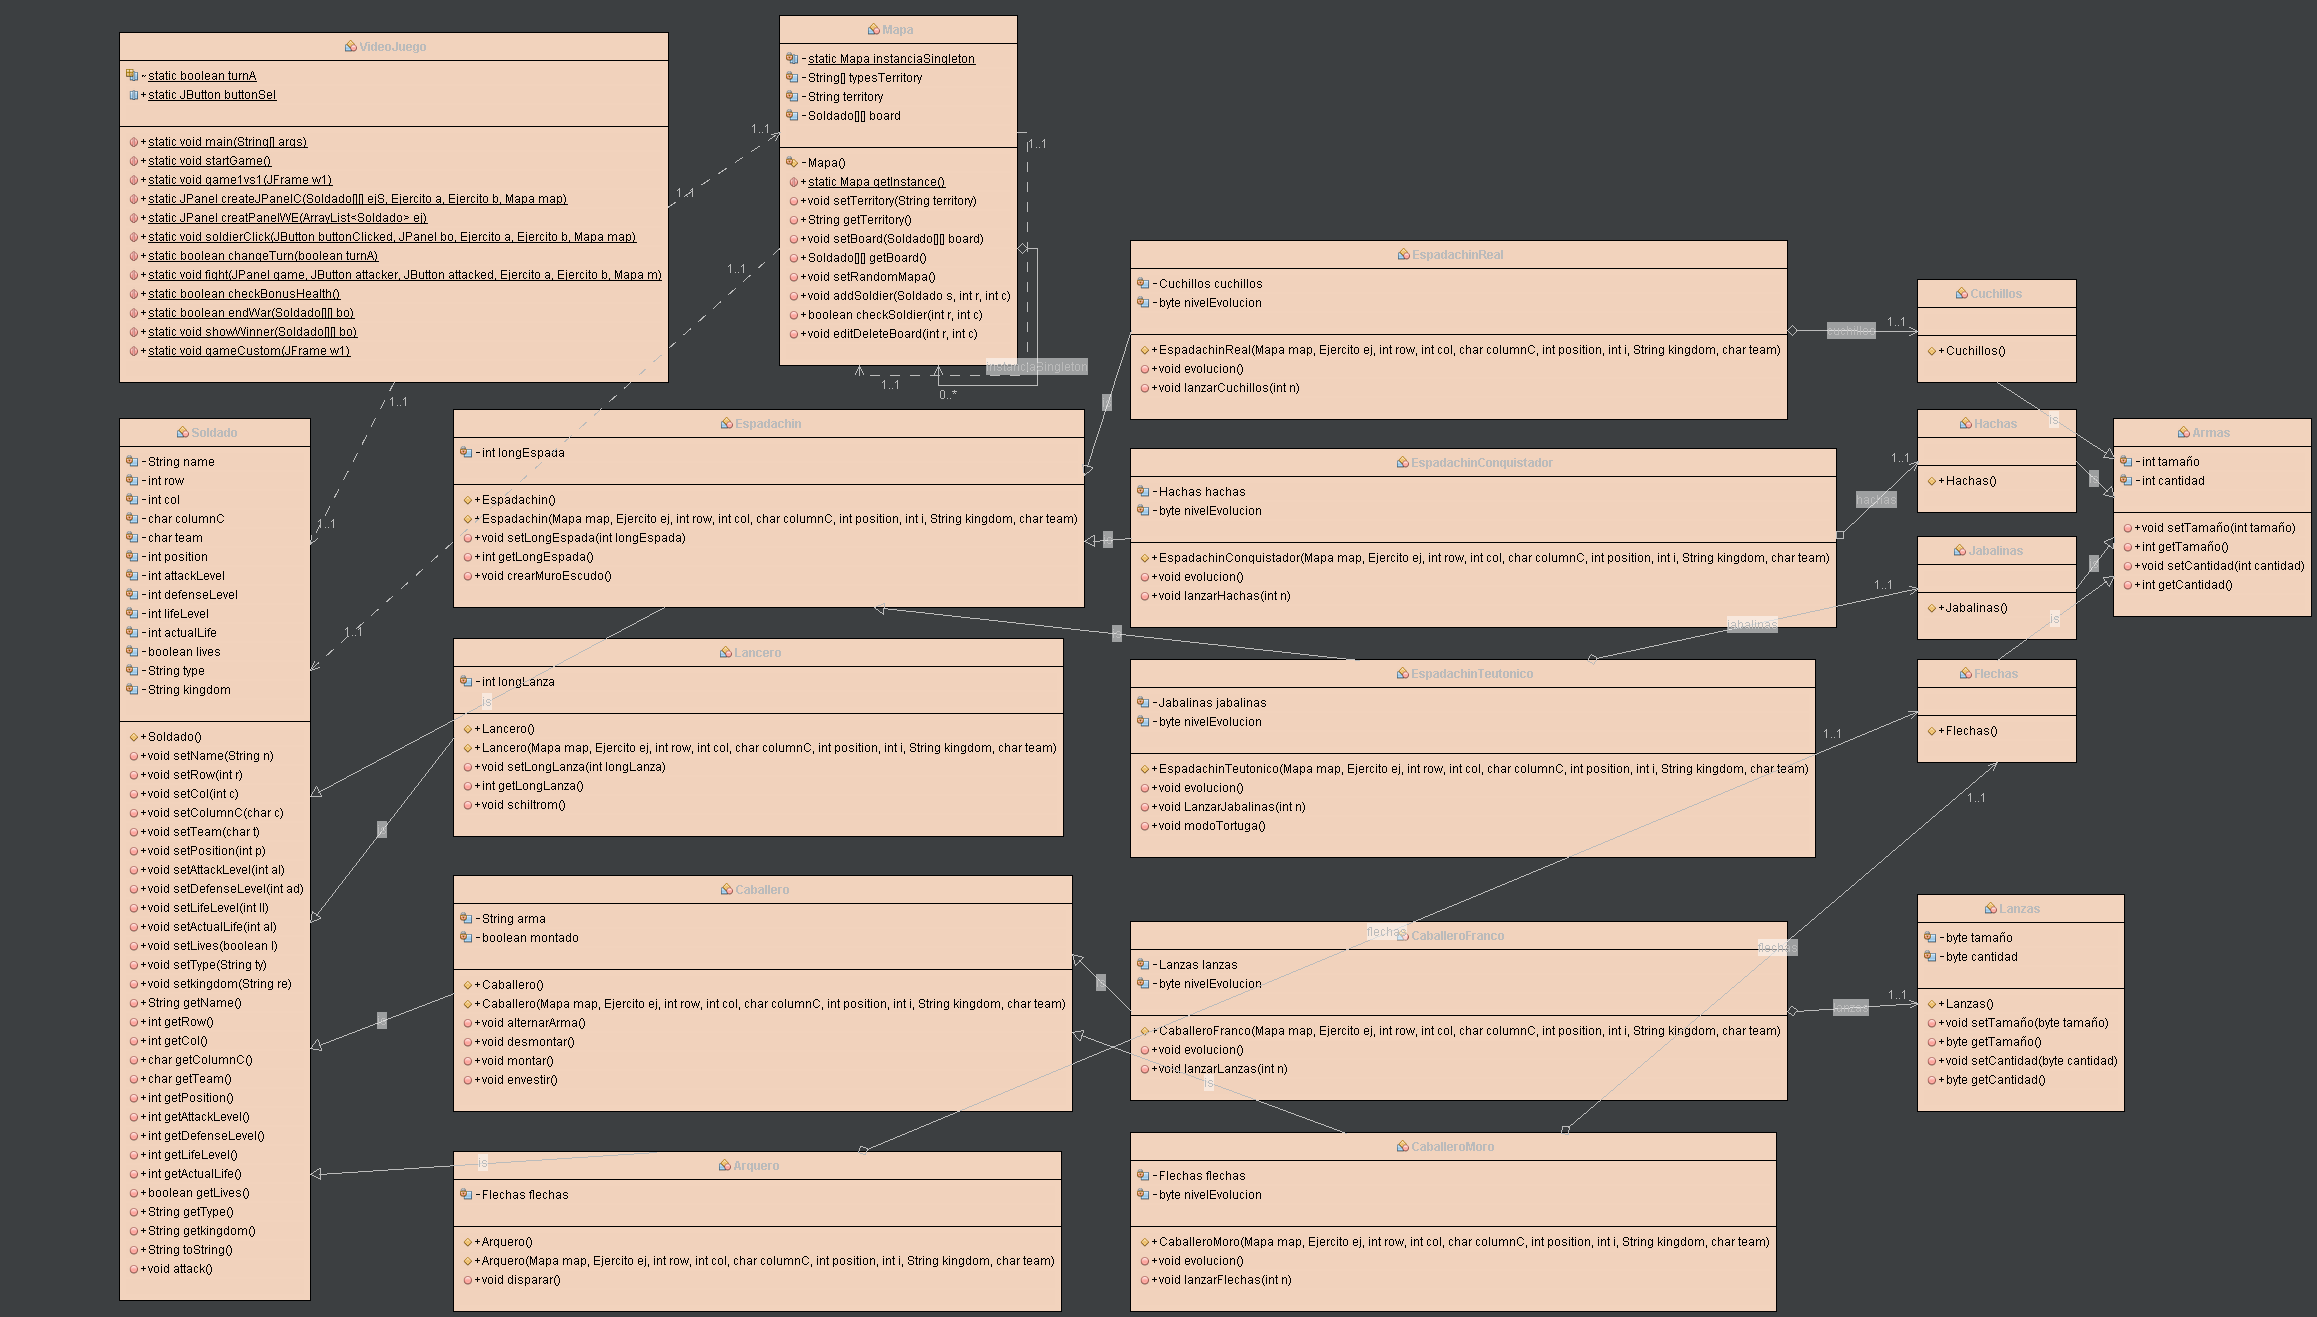
\includegraphics[width=1.1
    \textwidth,keepaspectratio]{img/22uml.png}
    \caption{}
\end{figure}

\href{https://github.com/hernanchoquehuanca/fp2-23b/blob/main/fase03/lab22/latex/img/22uml.png}{Aquí} Diagrama UML 22 para acceder al diagrama UML del repositorio y se observe con más claridad.

%------------------------------ ESTRUCTURA DE LABORATORIO --------------------------

\newpage

\subsection{Estructura de laboratorio \itemPracticeNumber} %%CAMBIAR NUMERO DE LAB
\begin{itemize}	
	\item El contenido que se entrega en este laboratorio es el siguiente:
\end{itemize}

%---------------------------------------- TREE -------------------------------------

\begin{lstlisting}[style=ascii-tree]

    lab20
    |   Soldado.java
    |   VideoJuego.java
    |
    |───latex
        |   Informe_Lab22.pdf
        |   Informe_Lab22.tex
        |
        |───img
        |       22uml.png           
        |       logo_episunsa.png  
        |       logo_abet.png      
        |       logo_unsa.jpg      
        |       vj1.png           
        |       vj2.png           
        |       vj3.png           
        |       vj4.png           
        |       vj5.png           
        |
        |───src
            |   Armas.java
            |   Arquero.java
            |   Caballero.java
            |   CaballeroFranco.java
            |   CaballeroMoro.java
            |   Cuchillos.java
            |   Ejercito.java
            |   Espadachin.java
            |   EspadachinConquistador.java
            |   EspadachinReal.java
            |   EspadachinTeutonico.java
            |   Flechas.java
            |   Hachas.java
            |   Jabalinas.java
            |   Lancero.java
            |   Lanzas.java
            |   Mapa.java
            |   Soldado.java
            |   Team.java
            |   VideoJuego.java
            |───src
                    01game.png

\end{lstlisting}    

\section{\textcolor{red}{Rúbricas}}
	
\subsection{\textcolor{red}{Entregable Informe}}
	\begin{table}[H]
		\caption{Tipo de Informe}
		\setlength{\tabcolsep}{0.5em} % for the horizontal padding
		{\renewcommand{\arraystretch}{1.5} % for the vertical padding
		\begin{tabular}{|p{3cm}|p{12cm}|}
			\hline
			\multicolumn{2}{|c|}{\textbf{\textcolor{red}{Informe}}}  \\
			\hline 
			\textbf{\textcolor{red}{Latex}} & \textcolor{blue}{El informe está en formato PDF desde Latex,  con un formato limpio (buena presentación) y fácil de leer.}   \\ 
			\hline 
		\end{tabular}
	}
	\end{table}
	
\clearpage

%------------------------------ RÚBRICA DE EVALUACIÓN ------------------------------
 
\subsection{\textcolor{red}{Rúbrica para el contenido del Informe y demostración}}
\begin{itemize}			
	\item El alumno debe marcar o dejar en blanco en celdas de la columna \textbf{Checklist} si cumplió con el ítem correspondiente.
	\item Si un alumno supera la fecha de entrega,  su calificación será sobre la nota mínima aprobada, siempre y cuando cumpla con todos lo ítem.
	\item El alumno debe auto calificarse en la columna \textbf{Estudiante} de acuerdo a la siguiente tabla:
	
    \begin{table}[ht]
    	\caption{Niveles de desempeño}
    	\begin{center}
    		\begin{tabular}{ccccc}
        	\hline
        	& \multicolumn{4}{c}{Nivel}\\
        	\cline{1-5}
        	\textbf{Puntos} & Insatisfactorio 25\%& En Proceso 50\% & Satisfactorio 75\% & Sobresaliente 100\%\\
        	\textbf{2.0}&0.5&1.0&1.5&2.0\\
        	\textbf{4.0}&1.0&2.0&3.0&4.0\\
        	\hline
    		\end{tabular}
    	\end{center}
    \end{table}	
\end{itemize}

%------------------------------------ EVALUACIÓN -----------------------------------

\begin{table}[H]
    \caption{Rúbrica para contenido del Informe y demostración}
    \setlength{\tabcolsep}{0.5em} % for the horizontal padding
    {\renewcommand{\arraystretch}{1.5}% for the vertical padding
    %\begin{center}
    \begin{tabular}{|p{2.7cm}|p{7cm}|x{1.3cm}|p{1.2cm}|p{1.5cm}|p{1.1cm}|}
        \hline
        \multicolumn{2}{|c|}{Contenido y demostración} & Puntos & Checklist & Estudiante & Profesor\\
        \hline
        \textbf{1. GitHub} & Hay enlace URL activo del directorio para el  laboratorio hacia su repositorio GitHub con código fuente terminado y fácil de revisar. &2 &X &2 & \\ 
        \hline
        \textbf{2. Commits} &  Hay capturas de pantalla de los commits más importantes con sus explicaciones detalladas. (El profesor puede preguntar para refrendar calificación). &4 &X &4 & \\ 
        \hline 
        \textbf{3. Código fuente} &  Hay porciones de código fuente importantes con numeración y explicaciones detalladas de sus funciones. &2 &X &2 & \\ 
        \hline 
        \textbf{4. Ejecución} & Se incluyen ejecuciones/pruebas del código fuente  explicadas gradualmente. &2 &X &2 & \\ 
        \hline			
        \textbf{5. Pregunta} & Se responde con completitud a la pregunta formulada en la tarea.  (El profesor puede preguntar para refrendar calificación).  &2 &X &2 & \\ 
        \hline	
        \textbf{6. Fechas} & Las fechas de modificación del código fuente están dentro de los plazos de fecha de entrega establecidos. &2 &X &2 & \\ 
        \hline 
        \textbf{7. Ortografía} & El documento no muestra errores ortográficos. &2 &X &2 & \\ 
        \hline 
        \textbf{8. Madurez} & El Informe muestra de manera general una evolución de la madurez del código fuente,  explicaciones puntuales pero precisas y un acabado impecable.   (El profesor puede preguntar para refrendar calificación).  &4 &X &3 & \\ 
        \hline
        \multicolumn{2}{|c|}{\textbf{Total}} &20 & &19 & \\ 
        \hline
    \end{tabular}
    %\end{center}
    %\label{tab:multicol}
    }
\end{table}
\clearpage

%------------------------------ REFERENCIAS ------------------------------

\section{Referencias}
\begin{itemize}			
    \item \url{https://docs.oracle.com/javase%2F7%2Fdocs%2Fapi%2F%2F/javax/swing/package-summary.html}
    \item \url{https://docs.oracle.com/javase/tutorial/java/IandI/subclasses.html}
    \item \url{https://docs.oracle.com/javase/tutorial/java/IandI/polymorphism.html}
    \item \url{https://docs.oracle.com/javase/7/docs/api/java/awt/package-summary.html}
    \item \url{https://docs.oracle.com/javase/tutorial/java/javaOO/lambdaexpressions.html}
    
\end{itemize}	
	
%\clearpage
%\bibliographystyle{apalike}
%\bibliographystyle{IEEEtranN}
%\bibliography{bibliography}
\end{document}